%%% DOCUMENTCLASS
%%%-------------------------------------------------------------------------------

\documentclass[a4paper,11pt, onecolumn, openany]{memoir}

%%% PACKAGES
%%%------------------------------------------------------------------------------

% Język i czcionki
\usepackage[utf8]{inputenc} % If utf8 encoding
% \usepackage[lantin1]{inputenc} % If not utf8 encoding, then this is probably the way to go
\usepackage[T1]{fontenc}
\usepackage{polski}
\usepackage[polish]{babel}
\usepackage[final]{microtype} % Less badboxes
\usepackage{lmodern}
\usepackage{tgpagella}

% Bibliografia
\usepackage{natbib}

% \usepackage{kpfonts} %Font
% \usepackage{tikz} % Figures
\usepackage{graphicx} % Include figures
\usepackage{import}
\usepackage{gensymb}
\usepackage{tcolorbox}
\graphicspath{ {ilustracje/} }
\definecolor{titlepagecolor}{cmyk}{0.7,.30,0,.40}
\definecolor{miejscekolor}{cmyk}{0,0,1,.10}
\definecolor{code-gray}{gray}{0.95}
%%% PAGE LAYOUT
%%%------------------------------------------------------------------------------

\setlrmarginsandblock{0.15\paperwidth}{*}{1} % Left and right margin
\setulmarginsandblock{0.2\paperwidth}{*}{1}  % Upper and lower margin
\checkandfixthelayout


%%% INTERNAL HYPERLINKS
%%%-------------------------------------------------------------------------------

\usepackage{hyperref}   % Internal hyperlinks
\hypersetup{
	pdfborder={0 0 0},      % No borders around internal hyperlinks
	pdfauthor={Tomasz Nycz} % author
}
\usepackage{memhfixc}   %

%%% THE DOCUMENT
%%% Where all the important stuff is included!
%%%-------------------------------------------------------------------------------

\author{Tomasz Nycz}
\title{Formaty i relacje przestrzenne w QGIS}

\usepackage{lipsum} % Just to put in some text

\begin{document}

	\frontmatter

	\maketitle


\mainmatter
\part{Odniesienia przestrzenne}
	\chapter{Zbiory danych przestrzennych}
		\section{Wymagania prawne}
		Podstawowe wymagania prawne dla przechowywania, przetwarzania informacji przestrzennej są zdefiniowane w rozporządzeniu
Rady Ministrów z dnia 12 kwietnia 2012 r. w sprawie Krajowych Ram Interoperacyjności, minimalnych wymagań dla rejestrów publicznych i wymiany informacji w postaci elektronicznej oraz minimalnych wymagań dla systemów teleinformatycznych (tekst jednolity Dz.U. 2017.247) oraz.


		W załączniku nr 2 rozporządzenia znajdujemy następujące istotne dla nas zapisy:  
		,,A. W celu wymiany zasobów informacyjnych przez podmioty realizujące zadania publiczne stosuje się:\\
		2. do danych zawierających informację graficzną stosuje się co najmniej jeden z następujących formatów danych:\\
		(2.3) .geotiff
		B. Do określenia struktury i wizualizacji dokumentu elektronicznego stosuje się następujące formaty danych:\\
		Do definiowania układu informacji polegającego na określeniu elementów informacyjnych oraz powiązań między nimi stosuje się następujące formaty danych:\\
		(1.1) .xml\\
		(1.2) .xsd\\
		(1.3) .gml''\\
	W dalszej części znajduje się informacja o formatach które ,,organ publiczny'' powinien móc obsłużyć w trybie do odczytu, a więc przyjmować od interesantów. 	
			\subsection{GML}
			XML (Extensible Markup Language, rozszerzalny język znaczników) to uniwersalny język znaczników przeznaczony do reprezentowania różnych danych w strukturalizowany sposób. Geography Markup Language to oparty na XML (eXtensible Markup Language) język opracowany przez Open Geospatial Consortium do transferu danych geograficznych. GML jest językiem formalnym służącym do opisu danych geograficznych zgodnie z zasadami opisanymi w normie ISO 19136:2007. Intencją opracowania języka GML była wymiana danych pomiędzy różnymi aplikacjami systemów informacji geograficznej. Struktura dokumentu GML, opisywana jest przez plik schematu – najczęściej XSD (XML Schema Description). Otwieranie formatu GML w środowisku QGIS (korzystającym w tym celu z biblioteki GDAL/OGR) jest proste, pod warunkiem jednak, że twórca zbioru przestrzega norm. Niestety w przypadku polskich danych przestrzennych często możemy się spotkać z bardzo luźnym podejściem. Wtedy pomaga przetworzenie takiego zbioru przy pomocy pakietu GDAL/OGR i jego sterownika GMLAS, z wykorzystaniem schematu aplikacyjnego XSD (schematy takie możemy znaleźć m.in. na stronach GUGiK). 			
		\section{GeoPackage - następca Shapefile}
		    Format danych Shapefile powstał na początku lat 90 XX wieku, opracowany przez firmę ESRI na potrzeby ArcView. Składa się on z co najmniej 3 plików (.shp, .shx, .dbf), lecz ich liczba może sięgać 14 - dla jednej warstwy danych. Uszkodzenie choćby jednego z plików obowiązkowych powoduje bezpowrotną utratę informacji. Jednocześnie informacje o układzie współrzędnych i odwzorowaniu, a także kodowaniu znaków narodowych znajdują się w osobnych plikach. Jak widać wygoda użytkowania takiego zbioru jest niewielka, ponieważ łatwo o utratę integralności.\\
		    W 2014 roku powstał standard OGC dla formatu danych przestrzennych GeoPackage. Utworzono go w oparciu o możliwości silnika bazy danych SQLite/Spatialite które pozwalają przechowywać wiele warstw danych o różnych typach geometrii, w tym również rastrów w postaci jednego pliku. W kolejnych latach powstawały rozszerzenia tego formatu pozwalające na przechowywanie w zbiorze GeoPackage również metadanych i informacji o projekcie. 
			\subsection{Tworzenie zbioru Geopackage}
			W oprogramowaniu QGIS sprowadza się do wybrania odpowiedniej pozycji z menu (Warstwa - Twórz warstwę - Nowa warstwa GeoPackage) lub paska narzędziowego, albo skorzystanie ze skrótu klawiszowego Ctrl+Shift+N. W nowo otwartym oknie musimy wprowadzić nazwę pliku na dysku w którym dane będą zapisywane, nazwę warstwy wektorowej, typ geometrii, oraz nazwy i typy pól danych. 
			\begin{figure}[!ht]
				\centering
				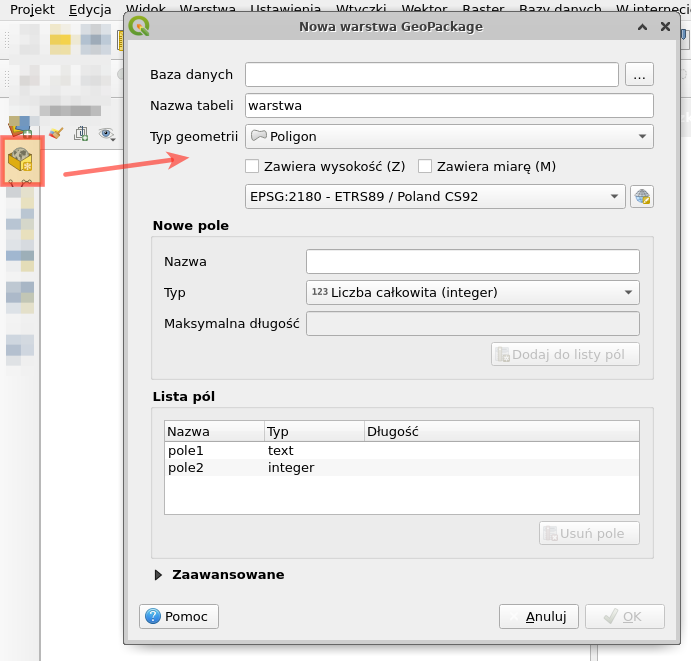
\includegraphics[width=7cm]{geopackage-tworz}
				\caption{Tworzenie nowej warstwy Geopackage}
			\end{figure}			
		    Istnieje również możliwość dodania opisu warstwy (komentarza), a także zmiana nazw pól identyfikatora (fid) czy kolumny geometrii. Są to ustawienia zaawansowane, na codzień nie ma potrzeby ingerencji w tą część.
			\subsection{Połączenie ze zbiorem}
			Jeśli planujemy dłuższą pracę z jakimś konkretnym zbiorem warstw danych, istnieje możliwość utworzenie połączenia do bazy. W tym celu musimy skorzystać z narzędzia znajdującego się w menu Baza Danych - Zarządzanie bazami danych. W oknie menedżera baz po lewej stronie znajdziemy listę tzw. dostawców. Są to sterowniki dostępu do GeoPackage, PostgreSQL, Oracle, MS Spatial, etc.
			\begin{figure}[!ht]
				\centering
				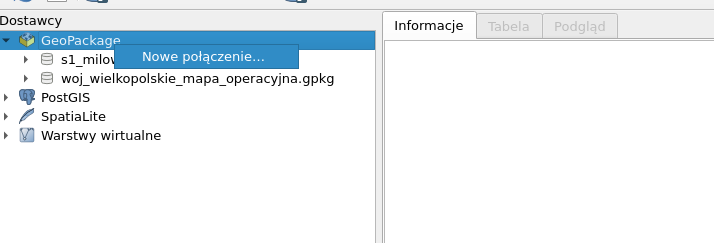
\includegraphics[width=7cm]{geopackage-polaczenie}
				\caption{Nowe połączenie Geopackage}
			\end{figure}
			 Jeśli kliknięmy w GeoPackage prawym klawiszem pojawi się opcja Nowe Połączenie. Należy jedynie wskazać plik .gpkg na dysku. Tak podłączona baza danych da nam wiele możliwości. Zobaczmy jakie.
		\section{Baza danych w GeoPackage}
			\subsection{Dodawanie wielu warstw}
			Do istniejącego zbioru GeoPackage możemy dodać więcej niż jedną warstwę danych. Wykonuje się taką operację poprzez wskazanie w oknie tworzenia lub zapisu warstwy istniejącego zbioru, ale ze wskazaniem innej nazwy tabeli.
			\begin{figure}[!ht]
				\centering
				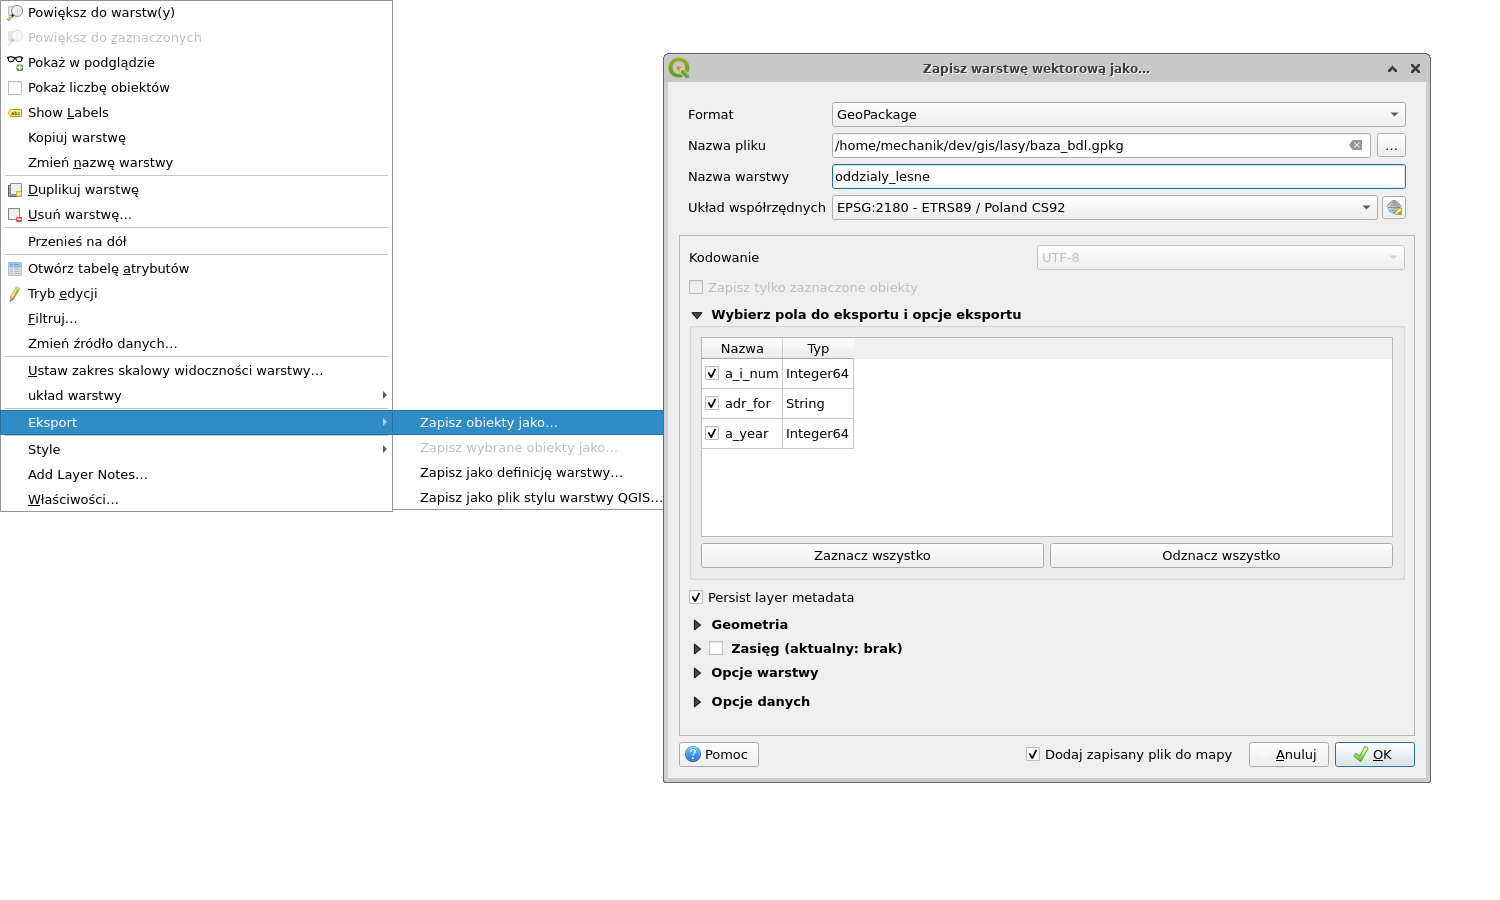
\includegraphics[width=15cm]{geopackage-zapisywanie}
				\caption{Zapisywanie warstwy do GeoPackage - menu kontekstowe oraz okno}
			\end{figure} 
			\subsection{Dołączanie projektu}
			Gotowy projekt można również zapisać do istniejącego, podłączonego jako baza danych zbioru GeoPackage. W tym celu należy wybrać menu Plik - Zapisz do - GeoPackage. W oknie należy w pierwszym polu wybrać z listy podłączoną bazę, zaś w drugim polu możemy dodać opisową nazwę projektu (może ona zawierać spacje, polskie znaki, może być dłuższa)
			\begin{figure}[!ht]
				\centering
				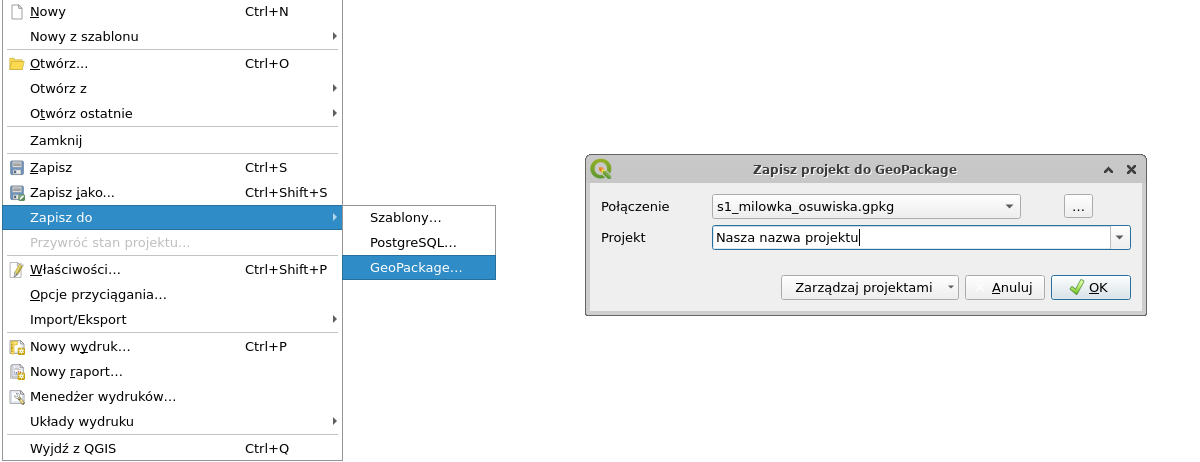
\includegraphics[width=15cm]{geopackage-zapis-projektu-menu}
				\caption{Zapisywanie projektu}
			\end{figure} 			
			
			\subsection{Dołączanie symboli i styli}
			Jeśli warstwa została otwarta z bazy danych GeoPackage istnieje możliwość zapisania stylu (kompozycji kartograficznej) warstwy do tejże bazy danych w celu ponownego wykorzystania. Musimy otworzyć okno Właściwości warstwy, w zakładce Styl w dolnej części okna znajdziemy klawisz Styl i możliwość zapisania (zobacz na ilustracji).
			\begin{figure}[!ht]
				\centering
				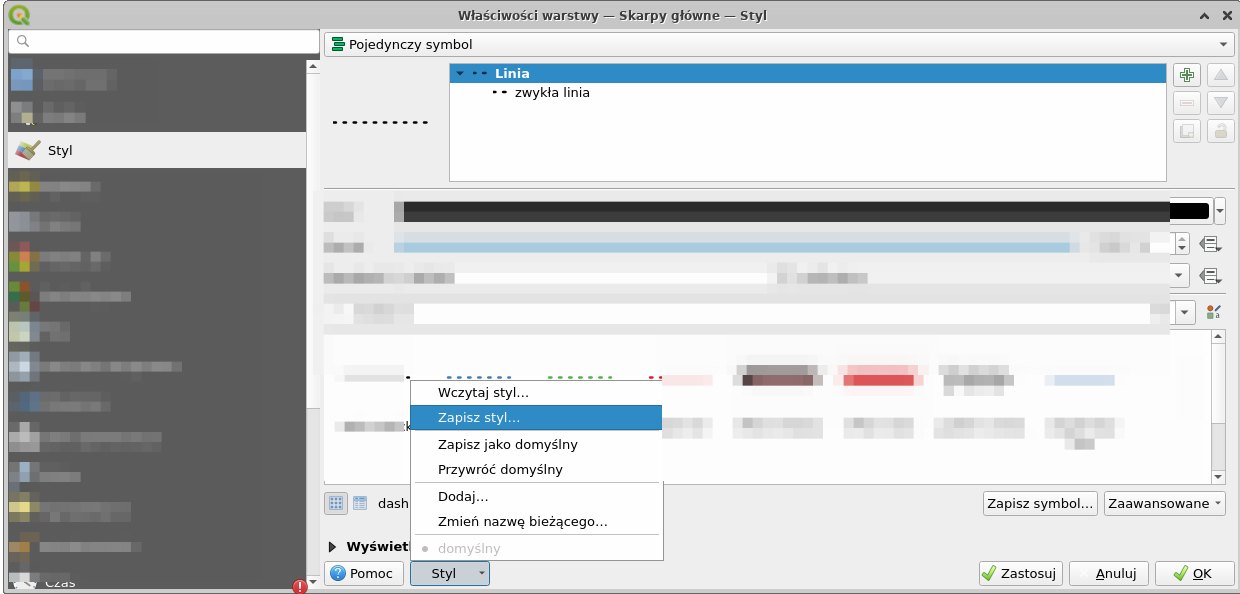
\includegraphics[width=7cm]{geopackage-styl}
				\caption{Zapisywanie stylu do zbioru Geopackage}
			\end{figure} 
			\subsection{Ćwiczenie - GeoPackage}
			\begin{itemize}
				\item Z katalogu modul1/geopackage/bdl zaczytamy dwie warstwy wektorowe w formacie Shapefile - F\_COMPARTMENT oraz F\_FOREST\_RANGE. 
				\item Następnie zapiszemy warstwę zasięgów leśnictw do nowego zbioru Geopackage (używając menu kontekstowego na liście warstw, oraz wskazując Eksport).
				\item Kolejno zapiszemy drugą z warstw do tego samego zbioru na dysku, pamiętając o nadaniu nazwy warstwy.
				\item Uruchamiamy menedżer baz danych (Menu Baza Danych - Zarządzanie bazami danych)
				\item W lewej części okna klikamy na napisie GeoPackage prawym klawiszem i dodajemy nowe połączenie. Następnie zamykamy okno menedżera baz.
				\item Z menu Projekt wybieramy Zapisz do - GeoPackage, a następnie zapisujemy projekt.
			\end{itemize}
	\chapter{Układy współrzędnych}
		\section{CRS i układ współrzędnych}
		W środowisku GIS możemy spotkać się z pojęciami CRS, odwzorowania kartograficznego, układu współrzędnych, oraz tzw. datum czy gridshift. Do dalszej komfortowej pracy konieczne jest zapoznanie się z nimi, oraz ich wzajemnymi powiązaniami.
		\begin{itemize}
			\item 		\textbf{Coordinate Reference System} - system odniesień przestrzennych. Jest to zbiór parametrów opisujących wszelkie cechy odniesień przestrzennych konieczne do poprawnego wskazania unikalnego miejsca w odniesieniu do powierzchni Ziemi. Należą do nich odwzorowanie kartograficzne, elipsoida, tzw. datum, południk i równoleżnik początkowy, oraz jednostki miary (stopnie, metry, sążnie, etc.)
			\item \textbf{Odwzorowanie kartograficzne} - jest to matematyczna realizacja sposobu odwzorowania elipsoidy obrotowej na płaszczyźnie mapy (lub zwizualizowania pseudo-trójwymiarowego w kartografii komputerowej). W praktyce europejskiej spotkamy się z odwzorowaniami: poprzecznym Merkatora, Gaussa-Kr\"{u}gera, azymutalnym Lamberta. W mapach obecnie archiwalnych popularne były również odwzorowania quasi-stereograficzne (WIG i GUGIK80) i Cassiniego-Soldnera. Można też było się spotkać z odwzorowaniami wielościennymi (np. wczesne edycje Messtichblatt).
			\item \textbf{Elipsoida} - to bryła powstała w wyniku obrotu elipsy wokół jej osi symetrii. Ziemię uznajemy w dużym uproszczeniu za elipsoidę obrotową (choć jej kształt jest dużo bardziej skomplikowany - nazywany geoidą). Ruch obrotowy Ziemi sprawia, że średnica równika jest o 43 km większa niż średnica pomiędzy biegunami. W czasach gdy kształt i rozmiary naszej planety były dopiero poznawane, powstało wiele opracowań opisujących parametry półosi wielkiej (a), półosi małej (b), oraz spłaszczenia (1/f). W naszych dalszych pracach będziemy wykorzystywać elipsoidy Bessela, Krassowskiego, oraz WGS84(GRS80).
			\item \textbf{Datum} - to geodezyjny układ odniesienia, opisujący kształt geoidy globalnie (np. systemy ETRS89/2000), jak również bardziej lokalnie (Pułkowo, Rauenberg, Hermannskogel). Obecnie w praktyce GIS geodezyjne układy odniesienia opisują translację względem geocentrycznego układu ETRF 89.
			\begin{figure}[!ht]
				\centering
				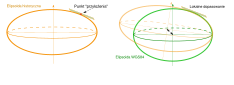
\includegraphics[width=15cm]{crs-transformacja-elipsoidy}
				\caption{Datum - Transformacja między układami odniesienia (za \citep{Affek_Georeferencing_2013})}
			\end{figure}
		    \item EPSG -  Rejestr i baza danych o układach odniesień (SRS i CRS), dawniej prowadzony przez \textbf{European Petroleum Survey Group}, obecnie Komitet Geomatyczny IOGP. Znajdują się w nim opisy parametrów elipsoid, południków zerowych, oraz całych CRS. Zamiennie z pojęciem kodu EPSG używa się terminu SRID - trochę szerszego, zawierającego również definicje własne producentów oprogramowania. Tabelę kodów EPSG przydatnych w codziennej pracy znajdziesz na końcu tego rozdziału. Można również skorzystać z wyszukiwarek kodu np. \hyperlink{https://epsg.org/search/map}{https://epsg.org/search/map}
		    \end{itemize}
	    Pozostałe parametry używane przy definiowaniu CRS opiszemy bezpośrednio przy stosowanych układach współrzędnych.

		\section{Uwarunkowania prawne}
		Wymagania prawne co do stosowanych układów odniesienia zdefiniowane są w rozporządzeniu Rady Ministrów z dnia 15 października 2012 r. w sprawie państwowego systemu odniesień przestrzennych (Dz.U. 2012 poz. 1247)\footnote{http://isap.sejm.gov.pl/isap.nsf/DocDetails.xsp?id=WDU20120001247}.
\begin{tcolorbox}[colback=black!5!white,colframe=white!55!black,title=§ 15. 1 i 2 rozporządzenia]
	§ 15. 1. Państwowy system odniesień przestrzennych stosuje się w pracach geodezyjnych i kartograficznych oraz przy
tworzeniu zbiorów danych przestrzennych przez organy władzy publicznej, przy czym:
\begin{enumerate}
	\item układ współrzędnych PL-LAEA stosuje się na potrzeby analiz przestrzennych i sprawozdawczości na poziomie ogólnoeuropejskim;
	\item układ współrzędnych PL-LCC stosuje się na potrzeby wydawania map w skali 1:500 000 i w mniejszych skalach;
	\item układ współrzędnych PL-UTM stosuje się na potrzeby wydawania standardowych opracowań kartograficznych w skalach od 1:10 000 do 1:250 000, wydawania map morskich oraz wydawania innych map przeznaczonych na potrzeby
	bezpieczeństwa i obronności państwa;
	\item układ współrzędnych PL-2000 stosuje się na potrzeby wykonywania map w skalach większych od 1:10 000 – w szczególności mapy ewidencyjnej i mapy zasadniczej.
\end{enumerate}
2. W pracach geodezyjnych i kartograficznych innych niż wymienione w ust. 1 pkt 1–4 stosuje się układ współrzędnych
PL-UTM lub układ współrzędnych PL-1992.
\end{tcolorbox}
			\subsection{PL-1992}
			Układ (w dalszej części skryptu będziemy używać nazwy układ 92) oparty jest o odwzorowanie Gaussa-Kr\"ugera z południkiem osiowym 19E. Praktyczna stosowalność układu między 14E i 24.30E. Współrzędna wschodnia (X) na południku osiowym przyjmuje wartość 500000, zaś współrzędna północna -5300000. Zniekształcenie skali na południku osiowym przyjmuje wartość 0,9993 (co przekłada się na skurcz -0,7m/km).
			\subsection{PL-2000}
			Układ PL-2000 (dalej w skrócie będziemy nazywać go 2000, ze wskazaniem strefy), tak jak układ 92 oparty jest o odwzorowanie Gaussa-Kr\"ugera, z tą różnicą że utworzono tu cztery strefy południkowe 15, 18, 21, 24 oraz przypisano im numery 5, 6, 7, 8. Współrzędna wschodnia na południku osiowym w każdej strefie przyjmuje wartość (500000 + n*1000000). Dla strefy 5 (15E) będzie to +5500000,00. Jak widzimy na podstawie pierwszej cyfry współrzędnej wschodniej możemy ustalić numer strefy. Współczynnik skali to 0,999923.
			\subsection{UTM, LAEA, LCC}
			Układ współrzędnych PL-LAEA oparty jest o odwzorowanie azymutalne równopowierzchniowe Lamberta, z południkiem początkowym 10E, równoleżnikiem 52N, współrzędne początkowe +4321000, +3210000.
			Układ współrzędnych PL-LCC oparty jest o odwzorowanie stożkowe równokątne Lamberta, z równoleżnikami siecznymi 35 i 65. Początek układu współrzędnych to punkt o współrzędnych geograficznych 10E, 52N i współrzędnych kartezjańskich + 4000000, +2800000.
			Układ PL-UTM to realizacja światowego układu współrzędnych UTM opartego o odwzorowanie poprzeczne Merkatora w trzech strefach południkowych z południkami 15, 21, 27 oznaczane odpowiednio numerami 33, 34, 35.
		\section{Starsze układy współrzędnych}
			Dawniej w naszym kraju stosowano wiele układów współrzędnych, o różnorodnych cechach. By wymienić choćby układ ,,42'' oparty oodwzorowanie Gaussa-Kr\"ugera, elipsoidę Krassowskiego z punktem przyłożenia w Pułkowie. Na jego podstawie opracowano największy zbiór map topograficznych w skali 1:10000 naszego kraju. Należy pamiętać że występował on w dwóch różnych wariantach stref odwzorowawczych (pasów południkowych) - 6 i 3 stopniowych. Strefy 6\degree obowiązywały przy realizacji map w skali 1:10000 i mniejszych.
			W późniejszym okresie stworzono układ współrzędnych 1965. Cechował się on występowaniem 5 stref odwzorowawczych, z których cztery zrealizowane były w odwzorowaniu quasi-stereograficznym, zaś strefa 5, obejmująca obszar dawnego (przed 1975 rokiem) województwa śląskiego w odwzorowaniu Gaussa-Kr\"ugera. W związku z tym na styku stref nie ma możliwości łatwego "sklejenia" arkuszy mapy. Mogą one cechować się innym obrotem, oraz innymi zniekształceniami odwzorowawczymi w punkcie. 
			\begin{figure}[!ht]
				\centering
				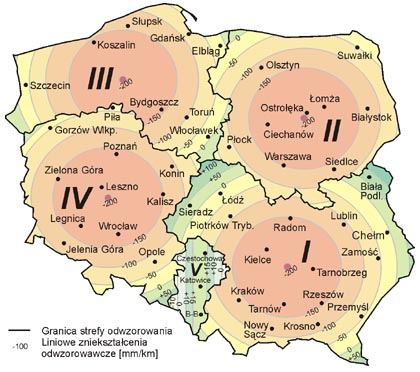
\includegraphics[width=8cm]{crs-1965-znieksztalcenia}
				\caption{Zniekształcenia odwzorowawcze stref układu 1965, źródło: Instrukcja O-1/O-2 z 2001 r.}
			\end{figure}
			W obiegu występują również mapy archiwalne w układzie Borowa Góra (w województwie śląskim zasób ten, w dyspozycji Archiwum Państwowego w Katowicach, we współpracy z Wojewódzkim Ośrodkiem Dokumentacji Geodezyjnej i Kartograficznej został przetworzony do usługi WMS w układzie 1992), układzie Sucha Góra (dokumentacja górnicza i dawne mapy topograficzne pruskie).
		\section{Identyfikatory i parametry - rozpoznawanie układu}	
			Aby ułatwić przyszłą pracę z układami współrzędnych w środowisku GIS zbierzemy tutaj niektóre parametry wspomnianych wcześniej układów\\
			\begin{tabular}{|c|c|}
				\hline
				Nazwa układu & Kod EPSG \\
				\hline
				Układ 1992 & 2180 \\
				\hline
				Układ 2000 & 2176,2177,2178, 2179 \\
				\hline
				Układ 1965&  3120 (I), 2172 (II), 2174 (III), 2174 (IV), 2175 (V)\\
				\hline
				Układ 1942 (strefy 3\degree)& 3329 (5/ 15\degree), 3330 (6/ 18\degree) 3331 (7/ 21\degree) 3332 (8/ 24\degree) \\
				\hline
				Układ 1942 (Pułkowo) strefy 6\degree& 3333 (3/ 15\degree), 3334 (4/ 21\degree) \\
				\hline
				LCC & 3034 \\
				\hline
				LAEA & 3035 \\
				\hline
				UTM & 32633 (33N), 32634 (34N)  \\
				\hline
				&  \\
				\hline
			\end{tabular}

		\section{Ćwiczenia}
		\subsection{Przypisanie CRS warstwy rastrowej}
		W tym ćwiczeniu wykorzystamy zbiory numerycznego modelu terenu w formacie ASCII GRID (.asc) udostępniane poprzez Główny Urząd Geodezji i Kartografii.
		W katalogu "/modul1/crs/dtm" znajdziemy przykładowe pliki w takim formacie. Otwieramy okno \textbf{Data Source Manager}, z paska narzędzi lub przy pomocy skrótu (Ctrl+L) i wskazujemy w zakładce przeglądarka nasz plik rastrowy z dysku.
		Zwróć uwagę na ikonkę \emph{znaku zapytania} znajdującą się po prawej stronie nazwy warstwy wyświetlanej na liście.
		\begin{figure}[!ht]
			\centering
			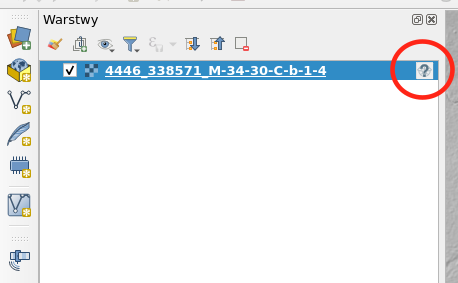
\includegraphics[width=10cm]{crs-cwiczenie1-brak-crs}
			\caption{Ostrzeżenie o braku zdefiniowanego CRS}
		\end{figure}
	Po najechaniu na ten symbol i kliknięciu otworzy się nam okno \textbf{Wybór układu współrzędnych}. W polu filtra możemy szybko odszukać potrzebny nam układ - w tym wypadku \emph{ETRS89 / Poland CS92} o kodzie EPSG:2180. Po zatwierdzeniu \emph{OK} wracamy do głównego okna mapy.
	\begin{figure}[!ht]
    	\centering
	    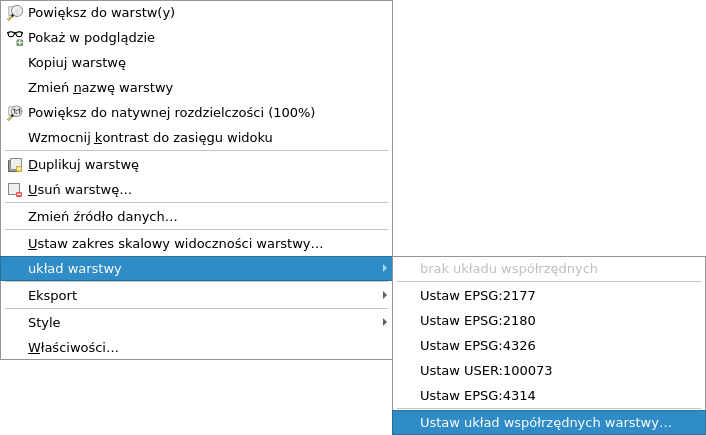
\includegraphics[width=10cm]{crs-cwiczenie1-menu-kontekstowe}
    	\caption{Menu kontekstowe warstwy - Ustawienie CRS}
    \end{figure}
		\subsection{Zmiana odwzorowania rastra}
				W kolejnym ćwiczeniu zmienimy odwzorowanie naszej warstwy rastrowej i zapiszemy nowy zbiór na dysku.
		Wykorzystamy uprzednio otwarty raster NMT. Nasze zadanie możemy wykonać na dwa sposoby. Pierwszym jest wykorzystanie algorytmu processingu \textbf{Zmień odwzorowanie}. Ukaże się nam okno algorytmu, w którym wskazujemy kolejno:
		\begin{enumerate}
			\item warstwę wejściową
			\item źródłowy układ współrzędnych
			\item docelowy układ współrzędnych
			\item metodę resamplingu
			\item możliwe jest zdefiniowanie wartości NODATA
			\item dodatkowe parametry GDAL (np. kafelkowanie, typ kompresji)
			\item czy warstwa wyjściowa ma być zapisana na dysk, czy tylko wyświetlona jako tymczasowa
		\end{enumerate}
		\begin{figure}[!ht]
		\centering
		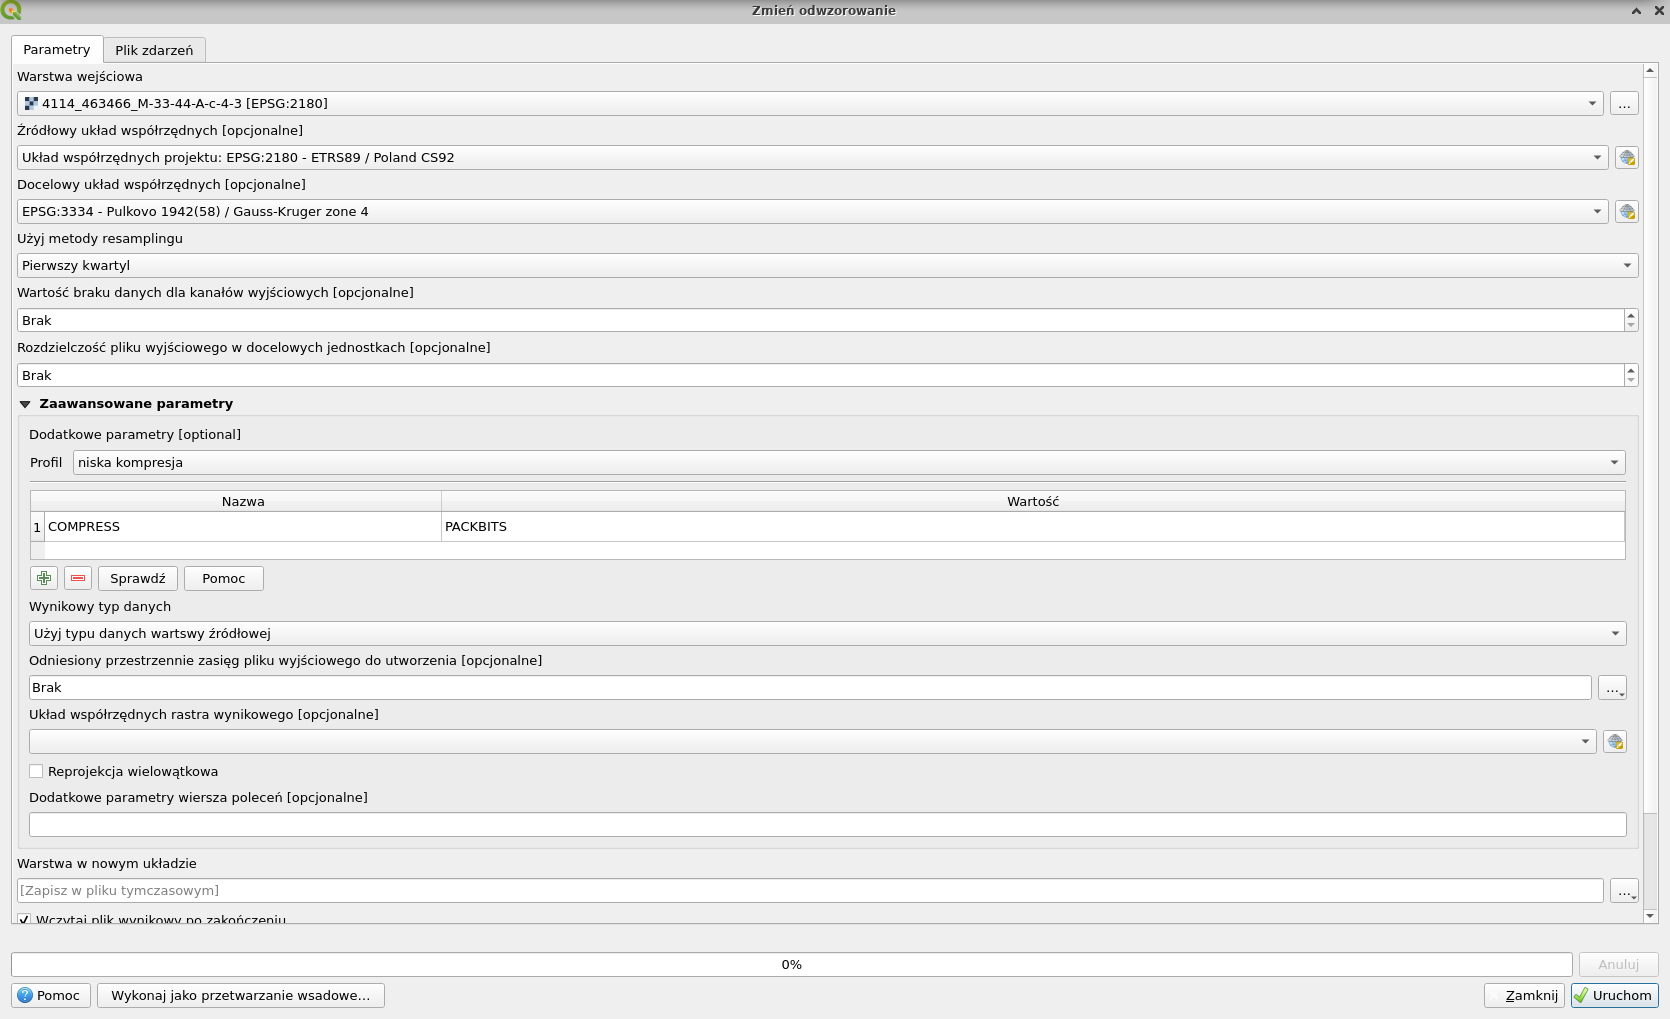
\includegraphics[width=10cm]{crs-cwiczenie2-zmien}
		\caption{Zmiana odwzorowania rastra}
	\end{figure}
		Po zatwierdzeniu następuje transformacja rastra, która zależnie od jego wielkości może potrwać nawet kilkadziesiąt sekund.
		Druga metodą polega na zapisaniu istniejącej warstwy przy pomocy menu kontekstowego Eksport -> Zapisz Jako.
	\begin{figure}[!ht]
	\centering
	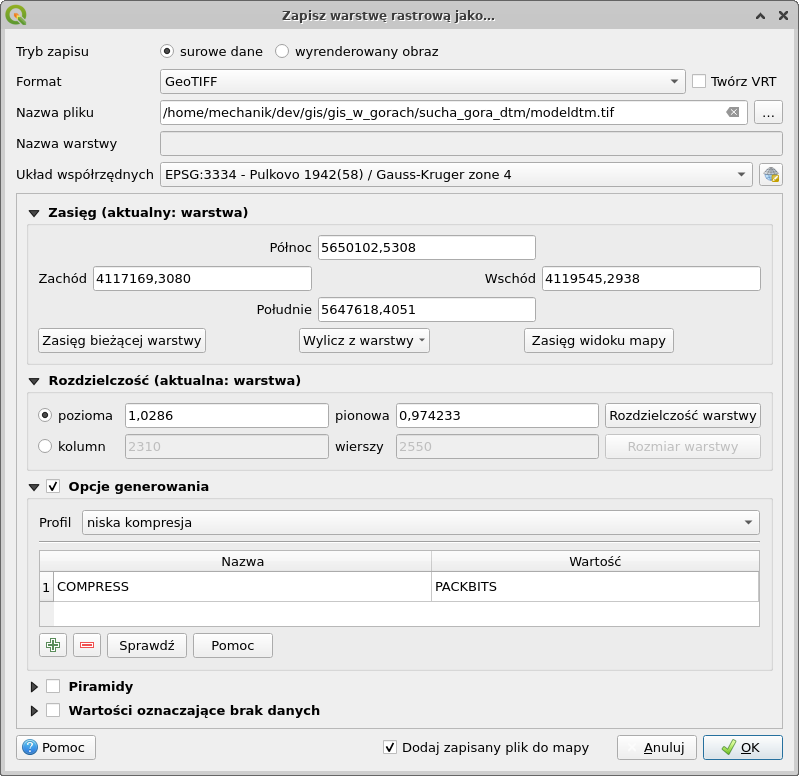
\includegraphics[width=10cm]{crs-cwiczenie2-zapisz-raster}
	\caption{Menu kontekstowe warstwy - Eksport Zapisz Jako}
\end{figure}
W tym wypadku również wskazujemy docelowy układ współrzędnych, ale także możemy wygodnie wskazać docelową rozdzielczość rastra.
	\subsection{Przypisanie układu współrzędnych wydruku}
	W ostatnim zadaniu tej sekcji przygotujemy arkusz wydruku mapy w odwzorowaniu azymutalnym Lamberta.
	\begin{enumerate}
		\item Zaczniemy w pustym projekcie, od załadowania zbioru \emph{/modul1/crs/prg/wojewodztwa.shp}. Są to granice województw pochodzące z Państwowego Rejestru Granic, w układzie współrzędnych 92.
		\item W kolejnym kroku uruchamiamy Menedżer wydruków i Nowy Wydruk (Ctrl+P)
		\begin{figure}[!ht]
			\centering
			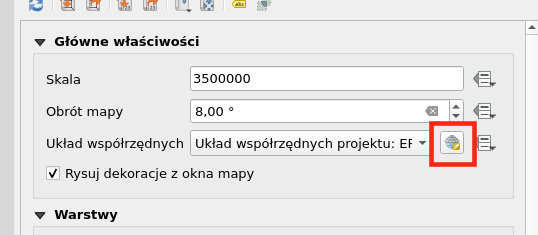
\includegraphics[width=5cm]{crs-wydruk-laea}
			\caption{Właściwości mapy - zmiana układu i skali}
		\end{figure}
		\item Na arkuszu osadzamy obiekt mapy, we właściwościach po prawej stronie ustawiamy skalę 1:3500000, oraz obrót 9 stopni, a następnie klikamy w symbol globusu poniżej (zobacz na ilustracji) i wskazujemy układ o symbolu EPSG:3035 (ETRS89-extended/LAEA Europe).
		\item W zakładce Siatka klikamy w ikonkę plusa, a następnie w przycisk Modyfikuj siatkę.
		\begin{figure}[!ht]
			\centering
			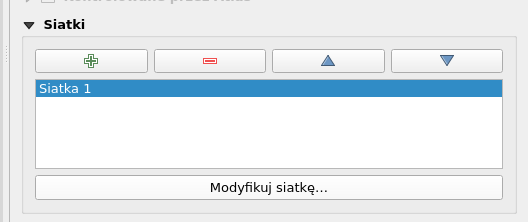
\includegraphics[width=5cm]{crs-laea-siatka}
			\caption{Zakładka Siatka - tworzenie nowej siatki kartograficznej}
		\end{figure}
		\item W ustawieniach Siatki (na ilustracji) wprowadzamy odstęp X i Y (wyrażony w jednostkach układu współrzędnych, tutaj metrach).
		\begin{figure}[!ht]
			\centering
			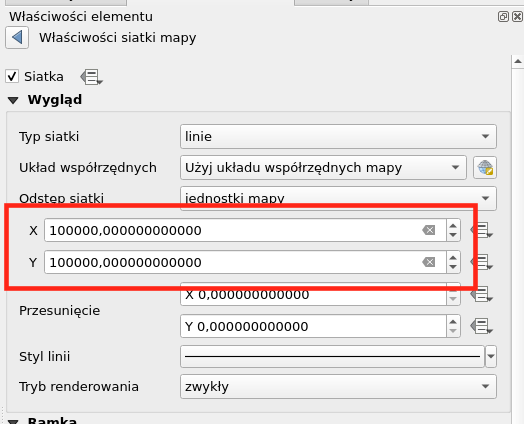
\includegraphics[width=5cm]{crs-laea-linie-siatki}
			\caption{Właściwości siatki}
		\end{figure}
		\item Na koniec zmieńmy odwzorowanie naszej mapy na stożkowe Lamberta (w oknie filtra wyboru układu użyjemy EPSG:3034, ETRS89-extended/LCC Europe), oraz skalę na 1:15000000, aby stwierdzić zniekształcenie linii południkowych.
	\end{enumerate}

	\chapter{Praca z archiwalnymi rastrami}
		\section{Wprowadzenie}
W niektórych przypadkach do prac w projekcie musimy dołączyć dane starsze, nie wytworzone w systemie GIS - np. tradycyjne mapy topograficzne, górnicze, czy plany i szkice. Aby tu uczynić musimy wykonać operację nadania georeferencji rastra, nazywanej również kalibracją rastra. W wyniku tej operacji do pliku w formacie GeoTIFF oprócz informacji graficznej dołączona zostanie również informacja o współrzędnych geograficznych narożników obrazu. Jeśli jednak dane archiwalne cechują się niską jakością (np. źle wykonane skanowanie mapy), konieczne będzie w tym kroku również jej wpasowanie w taki sposób, aby współrzędne w obrębie całego arkusza zmieniały się liniowo.
Całość tych zadań realizuje wtyczka Georeferencer GDAL, która w standardowej instalacji QGIS jest domyślnie zainstalowana i aktywowana. Odnaleźć ją możemy w menu Raster.
Jeśli uruchomimy wtyczkę i przejdziemy do ustawień przekształcenia (ikonka trybiku, lub menu Ustawienia), możemy zauważyć że do naszej pracy będziemy potrzebowali pewnych informacji. Pierwszą jest docelowy układ współrzędnych. Warto tu zaznaczyć, że nie musimy on być zbieżny z układem współrzędnych i odwzorowaniem pierwotnym. Pod warunkiem odpowiedniej ilości punktów kontrolnych, operacja transformacji graficznej może dać całkiem dobre wyniki. Kolejną jest typ przekształcenia z następującymi cechami:\\
		\begin{tabular}{|p{0.2\textwidth}|p{0.6\textwidth}|p{0.1\textwidth}|}
	\hline
	Typ & Opis & Ilość GCP \\
	\hline
	Liniowa & Podstawowy, najprostszy tryb, polegający wyłącznie na translacji, bez zmiany skali i obrotu. & 3 \\
	\hline
	Helmerta & Transformacja Helmerta w jej klasycznej postaci, to jest translacja wraz ze zmianą skali i obrotem. Przy dobrej jakości skanie, oraz zgodności odwzorowań pierwotnego i docelowego, jest to metoda najszybsza. & 4 \\
	\hline
	Wielomiany 1-3 & Transformacja wielomianowa jest najczęściej stosowaną. Wielomian drugiego stopnia pozwala na wprowadzenie poza zmianami opisanymi w transformacji Helmerta, również krzywiznę.  & 5-10 \\
	\hline
	Funkcja sklejana (TPS) & Thin Plate Spline pozwala na wyrównywanie lokalnych deformacji, szczególnie przy bardzo złej jakości skanach. & 3 \\
	\hline
	Odwzorowane (rzutowe) & Tryb podobny do liniowego, z możliwością obrotu & 3 \\
	\hline
		\end{tabular}\\
			\begin{figure}[!ht]
			\centering
			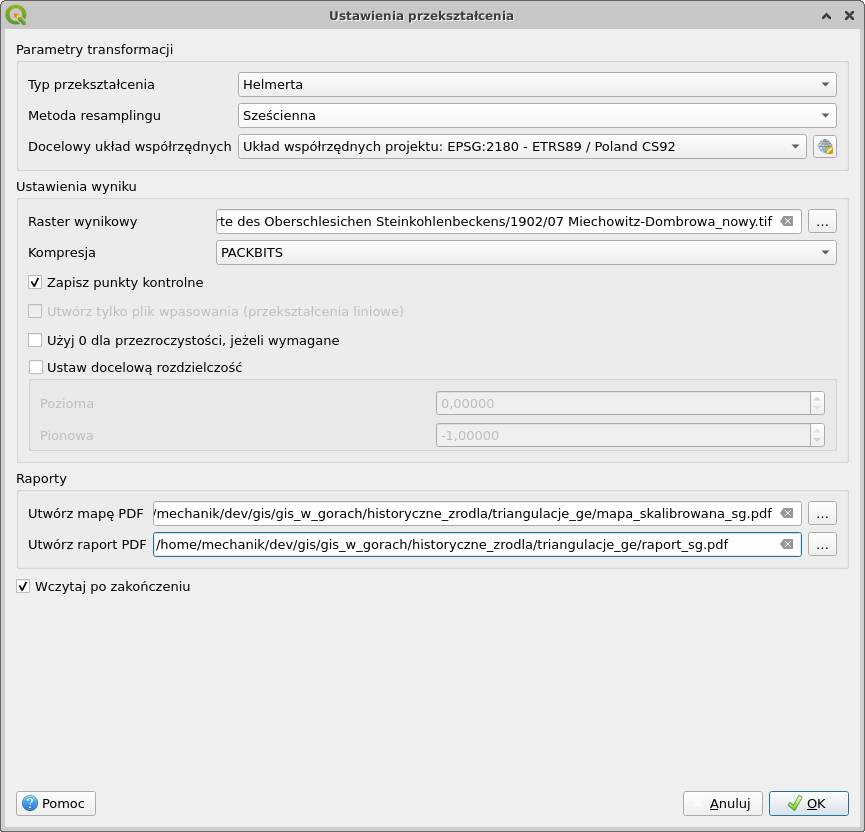
\includegraphics[width=10cm]{georef-ustawienia}
			\caption{Ustawienia przekształcenia}
		\end{figure}
Punkty kontrolne (GCP) możemy wprowadzać w oparciu o współrzędne numeryczne lub poprzez wskazanie na mapie współczesnej (warstwie rastrowej lub wektorowej o wcześniej nadanej georeferencji). Szczególnym rozwinięciem tej drugiej metody jest kalibracji na ,,narożniki mapy''.

		\section{Referencja do punktów wspólnych}
		Podstawowa metoda wyznaczania punktów kontrolnych to zaznaczenie punktu na mapie archiwalnej i wprowadzenie w pojawiającym się oknie współrzędnych, lub wskazanie ,,Z obszaru mapy'' czyli z materiału współczesnego, z nadaną georeferencją.
		\begin{figure}[!ht]
			\centering
			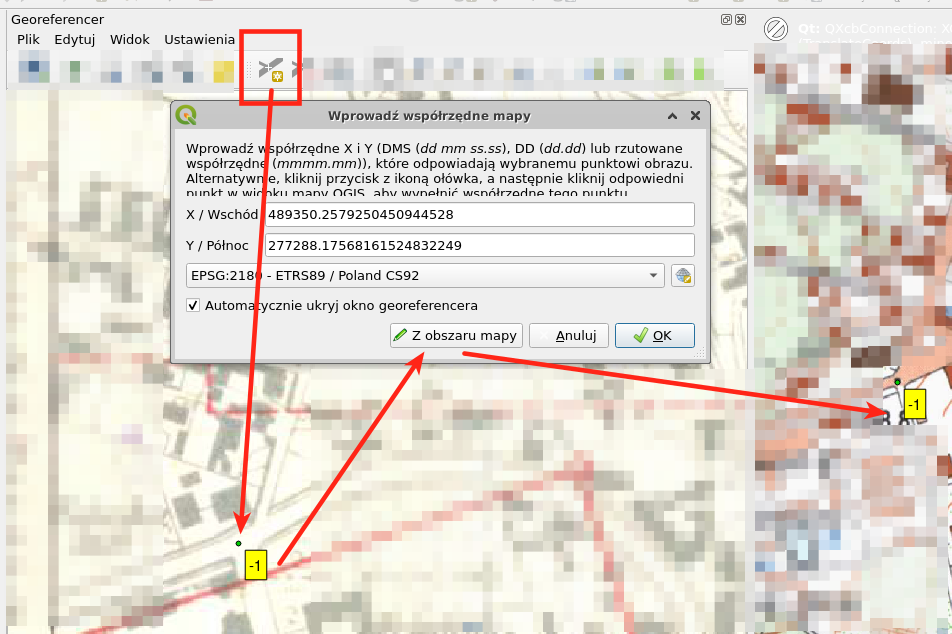
\includegraphics[width=10cm]{georef-dodaj}
			\caption{Dodawanie punktu}
		\end{figure}
		Po dodaniu odpowiedniej ilości punktów, zależnie od metody transformacji, możemy zobaczyć informację o błędzie średnim kalibracji, oraz przesunięciach dx, dy konkretnych punktów. Na podstawie tabeli możemy podjąć decyzję o poprawie lokalizacji punktu, lub jego usunięciu jako niepewnego.
		\begin{figure}[!ht]
		\centering
		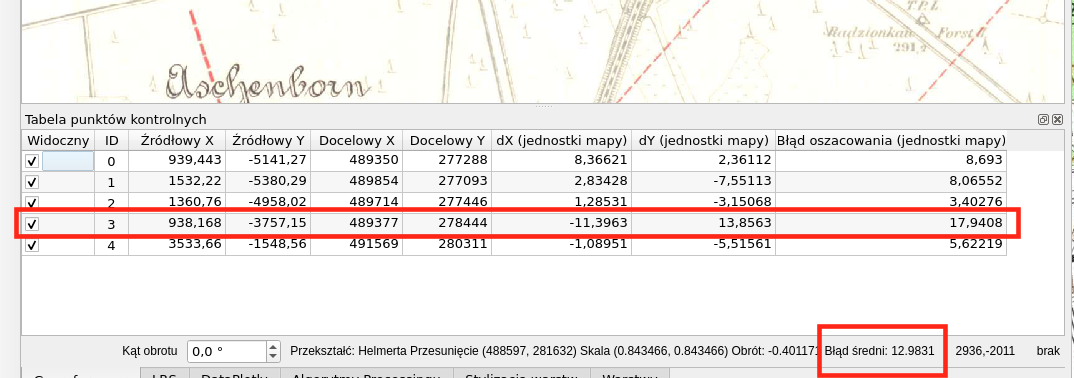
\includegraphics[width=10cm]{georef-tabela-punktow}
		\caption{Tabela punktów kontrolnych}
	\end{figure}

		\section{Referencja do narożników mapy}
		Druga z metod pracy polega na wstępnym przygotowaniu siatki skorowidzowej, z punktami w współrzędnych narożników mapy. Ta metoda doskonale sprawdza się przy kalibracji map seryjnych, np. geologicznych, czy dawnych Messtichblattach, przy założeniu że skan mapy został wykonany przy dużej staranności (brak skurczu papieru, pofalowań, w miarę możliwości utrzymanie pionu).
		Przy takich założeniach sprawdzamy rozpiętość przestrzenną arkusza i przy pomocy narzędzia \textbf{Siatka} z menu Wektor -> Analiza tworzymy siatkę prostokątów, w układzie współrzędnych dawnej mapy, z wskazaniem współrzędnych początkowych, oraz offsetu.
		Następnie włączamy przyciąganie do obiektów (menu Projekt -> Ustawienia Przyciągania) i wskazujemy jako miarę przyciągania np. 10 px. To pozwoli na bardzo sprawne i szybkie dodawanie nowych punktów, a w konsekwencji bardzo wydajną pracę.
		\pagebreak
		\section{Ćwiczenia}
		\subsection{Kalibracja dawnej mapy górniczej}
		W tym ćwiczeniu skalibrujemy dawną mapę górniczą Głównej Kluczowej Sztolni Dziedzicznej, która wykonana była w odwzorowaniu Cassiniego, ale bez wskazanych współrzędnych, nie znamy też układu. Konieczne więc będzie zastosowanie metody kalibracji na punkty wspólne.

		\begin{enumerate}
		\item Uruchamiamy Georeferencer z menu Raster
		\item W ustawieniach przekształcenia wskazujemy układ współrzędnych PUWG 1992 (CS92 Poland, EPSG:2180)
		\item Jako metody przekształcenia użyjemy Helmerta
		\item W oknie głównym mapy otworzymy warstwę WMS mapy topograficznej i przybliżymy na obszar Zabrza
		\item Poprzez obserwację mapy oryginalnej i współczesnej wyszukamy punkty wspólne (co najmniej 5)
		\item W ustawieniach przekształcenia wskażemy plik docelowy, plik raportu i plik mapy pdf, oraz konieczność otworzenia warstwy po zakończeniu
		\item Zatwierdzamy nasze przekształcenie symbolem zielonego trójkąta (Play)
		\end{enumerate}
    \subsection{Kalibracja mapy seryjnej na siatkę}
W tym przypadku wykorzystamy dwa arkusze seryjnej Szczegółowej Mapy Geologicznej PIG \hyperlink{http://geologia.pgi.gov.pl/}{http://geologia.pgi.gov.pl/} wykonane w oparciu o układ 42 i cięcie Międzynarodowej Mapy Świata. Nosi ona oznaczenia zarówno siatki kilometrowej w układzie 42 jak i współrzędnych geograficznych. Na tej podstawie przygotujemy w pierwszej kolejności siatkę prostokątów skorowidzu. Później przechodzimy do samej kalibracji. 
		\begin{enumerate}
		\item W menu Projekt uruchamiamy Ustawienia przyciągania
		\item Wprowadzamy ustawienie przyciągania do wierzchołków, oraz odległość 10 pikseli
		\begin{figure}[!ht]
			\centering
			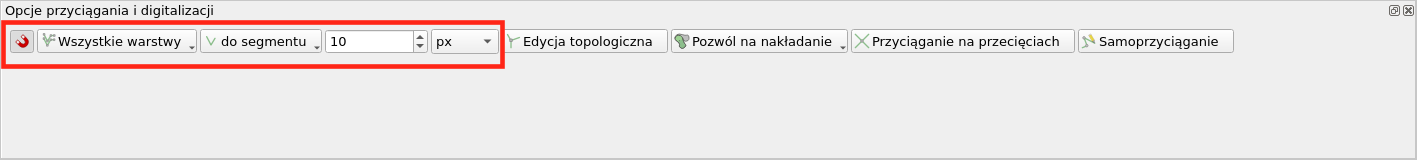
\includegraphics[width=10cm]{georef-przyciaganie}
			\caption{Ustawienia przyciągania}
		\end{figure}
		\item Uruchamiamy narzędzie \textbf{Utwórz Siatkę} z menu Wektor -> Narzędzia badawcze
		\item Wprowadzamy parametry: Typ siatki Prostokąt (Poligon), Zasięg siatki \emph{18.50,19.0,50.3333,51.00 [EPSG:4326]}, Odstęp w poziomie 0,25  (czyli 15'), Odstęp w pionie 0,3333 (10'), pokrycie poziome i pionowe zostawiamy 0, wskazujemy układ współrzędnych EPSG:4326 i pozostałe pola pozostawiamy bez zmian
		\begin{figure}[!ht]
	\centering
	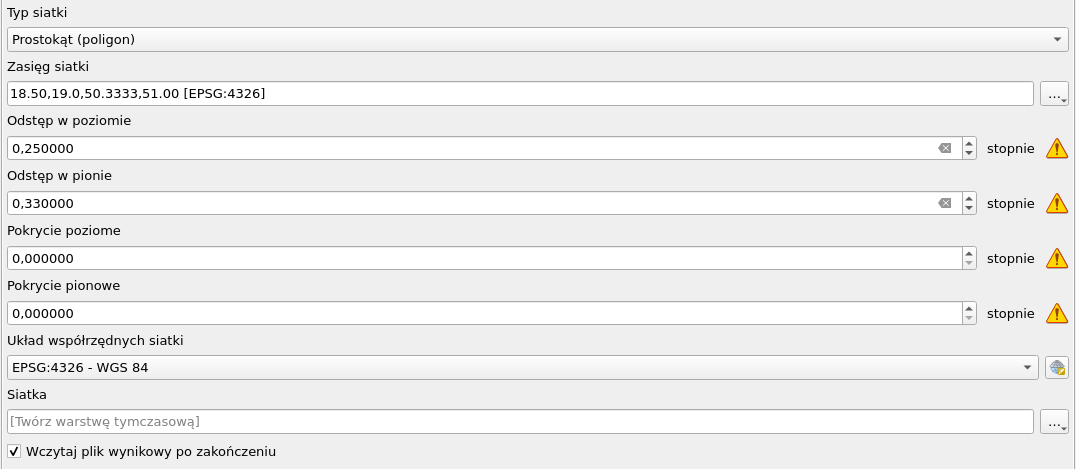
\includegraphics[width=10cm]{georef-siatka}
	\caption{Ustawienia przyciągania}
\end{figure}		
		\item W Georeferencerze GDAL z menu Plik wybieramy funkcję Resetuj Georeferencer
		\item Następnie otwieramy pierwszą z map znajdujących się w katalogu /modul1/georef/seryjne
		\item Wybieramy ustawienia przekształcenia, wprowadzamy nazwę pliku wynikowego, przekształcenie Wielomian 1
		\begin{figure}[!ht]
			\centering
			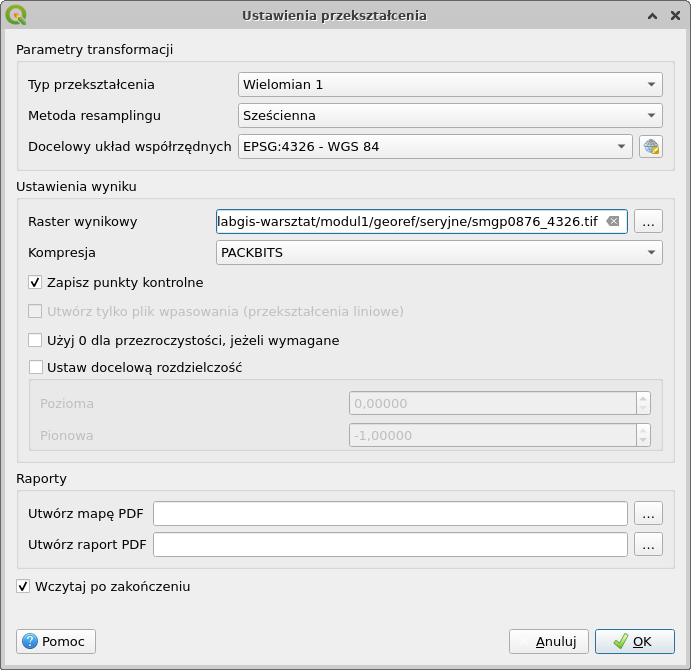
\includegraphics[width=8cm]{georef-ustawienia-skorowidz}
			\caption{Ustawienia przekształcenia}
		\end{figure}		
		\item Zaznaczamy kolejno cztery narożniki na mapie archiwalnej i w oknie mapy odpowiadający obiekt z siatki skorowidzowej.
		\item Zatwierdzamy zmiany przy pomocy Wykonaj przekształcenie
		\item Powtarzamy operację od punktu 5 dla drugiej z map
		\end{enumerate}

	\chapter{Referencja liniowa}
		\section{Wprowadzenie}
		W wcześniejszych ćwiczeniach poznaliśmy referencję przestrzenną w współrzędnych kartezjańskich XY. Istnieje możliwość dodania do naszych wektorowych zbiorów GIS również innych wymiarów - czasu, wysokości, czy pikietażu/kilometrażu. Ten ostatni parametr przechowuje się przy pomocy techniki nazywanej Linear Reference System (System Referencji Liniowej). Zakłada ona przygotowanie takiego zbioru w którym każdemu odcinkowi linii, (lub każdemu segmentowi) przypisuje się wartości współrzędnej M (measure) dla punktu początkowego i końcowego. Na tej podstawie możemy później odszukać dowolną lokalizację w ramach wskazanego odcinka. W praktyce budownictwa drogowego i kolejowego, ale również zarządzania siecią wodną, taki sposób określania lokalizacji jest podstawowym. Spójrzmy na przykład ogłoszenia przetargu na budowę drogi. 
		\begin{figure}[!ht]
			\centering
			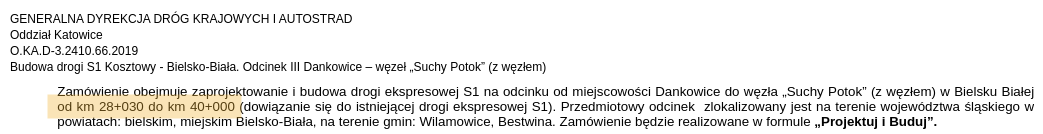
\includegraphics[width=11cm]{lrs-ogloszenie}
			\caption{Przykład ogłoszenia przetargu ze wskazanym kilometrażem}
		\end{figure}
	Podane są tu wartości kilometrów oraz metrów początku i końca opracowania dla drogi. 
		\section{Przygotowanie zbioru liniowego}
		 W wtyczce LRS taką operację wykonuje się w zakładce Kalibracja.  
		\section{Wyszukiwanie lokalizacji}
		\section{Ćwiczenia}
		\subsection{Kalibracja}
		\begin{enumerate}
			\item W nowym projekcie wczytujemy z pliku bielawa.gpkg w katalogu modul1/lrs obie warstwy wektorowe (jedna liniowa, druga punktowa).
			\item W wtyczce LRS przechodzimy do zakładki Kalibracja, a wewnątrz niej do zakładki Input.
			\item Wskazujemy w polu Warstwa liniowa naszą warstwę sieci drogowej, kolejowej lub wodnej.
			\item W polu Atrybut trasy - linie należy wskazać kolumnę z tabeli, w której znajdują się numery lub nazwy (np. dla rzek)
			\item W ten sam sposób wypełniamy pola dla Warstwy Punktowej i Atrybutu trasy - punkty.
			\item W polu Atrybut pikietażu wskazujemy kolumnę tabeli warstwy punktowej w której znajdują się wartości miary.
			\item Ostatnie pole w tej części wskazujemy jednostki miary - domyślne kilometry
			\item Wskazujemy wartość przyciągania punktów - 5 metrów
			\item Zaznaczamy również Ekstrapolacja
			\item Zatwierdzamy klawiszem OK
			\item Wprowadzamy nazwę warstwy wynikowej np. Linie z miarą i używamy klawisza Create
			\item W zakładce Błędy używamy przycisków w dolnej części - Create Error Layers, Create Quality Layers
			\item Przejrzymy teraz jakość naszej kalibracji w warstwie Quality (np. otwierając tabelę atrybutów)
		\end{enumerate}
			\begin{figure}[!ht]
		\centering
		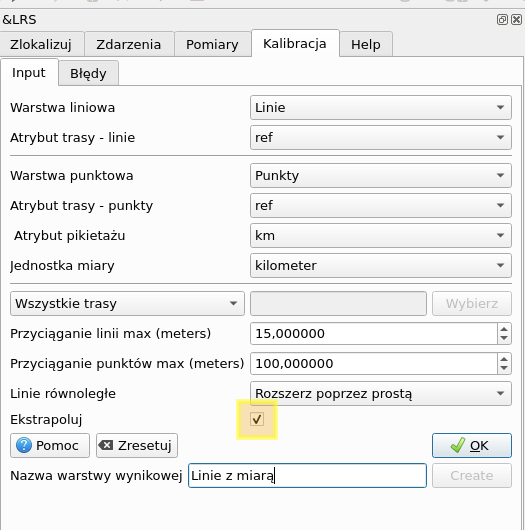
\includegraphics[width=8cm]{lrs-kalibracja}
		\caption{Ustawienia kalibracji}
	\end{figure}
\part{Analiza}
	\chapter{Numeryczny model terenu - wprowadzenie}
		Pojęciem \textbf{Numerycznego modelu terenu} (NMT) określamy zbiory danych przestrzennych najczęściej w formacie rastrowym, zawierające informacje o ukształtowaniu powierzchni terenu. Wraz z \textbf{Numerycznym Modelem Pokrycia Terenu} (NMPT) powstają obecnie z danych Lotniczego Skaningu Laserowego (ALS/LiDAR). Po klasyfikacji (przy pomocy filtrów morfologicznych) chmury punktów ALS uzyskuje się informacje o pokryciu terenu budynkami i budowlami, wysoką, średnią i niską roślinnością.
		\begin{equation}\label{rownanienmt}
		NMT = NMPT - Obiekty
		\end{equation}
		Z danych NMT możemy uzyskać wiele produktów pochodnych, wśród których najczęściej wykorzystywanymi są mapa spadków, ekspozycji, wskaźniki szorstkości, wskaźniki pozycji topograficznej. Zaprezentuję tutaj kilka z nich.

		\section{Mapa spadków}
		Mapa spadków przedstawia informację o największym nachyleniu pomiędzy sąsiadującymi komórkami rastra.
		W QGIS zainstalowanym z pakietu OSGEO4W możemy wygenerować mapę spadków przy pomocy biblioteki GDAL, pakietu GRASS lub SAGA GIS. Wszystkie te algorytmy są dostępne z poziomu narzędzi \emph{Processingu}.
		Podstawowym, najprostszym jest algorytm GDAL - znajdziemy go w grupie \emph{GDAL -> Raster-Analiza}.
		Do wyboru mamy tutaj:
		\begin{itemize}
			\item możliwość wskazania skali dla współrzędnej Z (np. gdy wyrażona jest w stopach)
			\item obliczenia przy granicach, czyli sposób obliczania wartości nachylenia dla tych komórek rastra, które ze względu na położenie nie są otoczone z każdej strony conajmniej jedną inną komórką.
			\item wyrażenie wartości spadku w procentach a nie stopniach. Polega to na założeniu że nachylenie, przy którym deniwelacja między dwoma punktami jest równa odległości kartezjańskiej, wynosi 100\%. Warunek taki spełniony jest dla kąta 45\degree.
			\item Formuła Zevenbergen-Thorne zamiast Horn'a. Pierwsza z nich lepiej sprawdza się w obliczeniach terenów o łagodnych zmianach powierzchni, zaś druga w warunkach bardzo zróżnicowanego krajobrazu. Formuła Horn'a używa tzw. okna 3x3.
		\end{itemize}
			\begin{figure}[!ht]
	\centering
	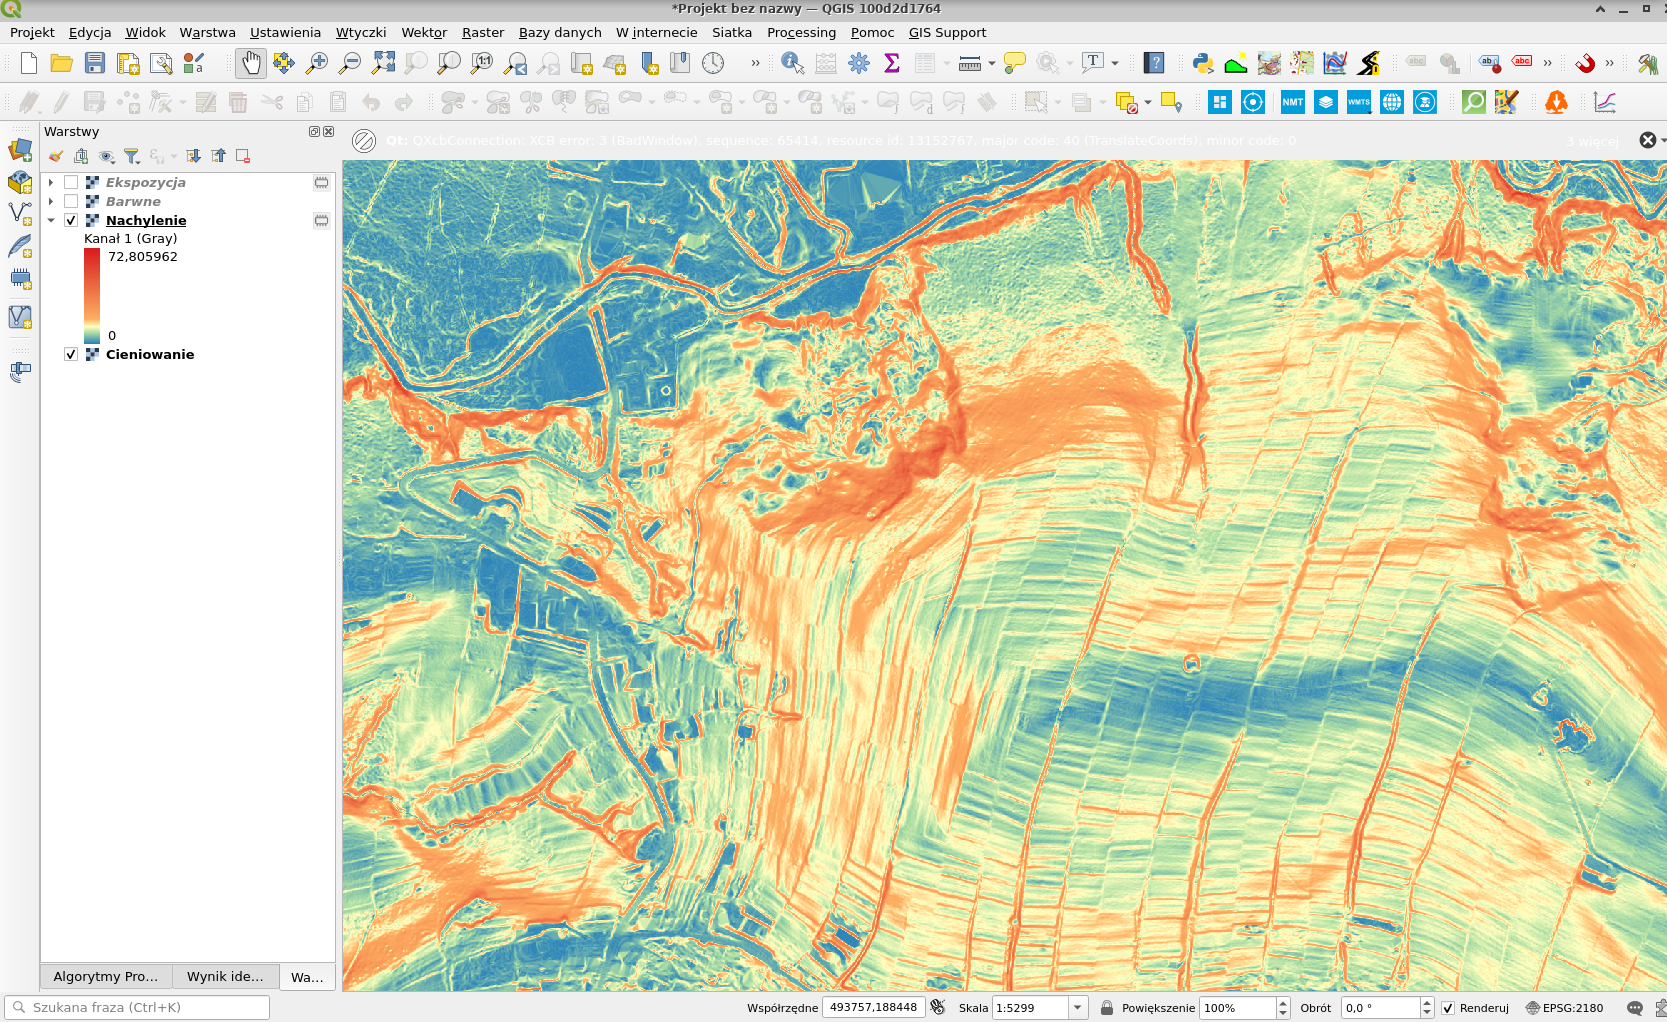
\includegraphics[width=10cm]{nmt-nachylenie}
	\caption{Mapa spadków}
\end{figure}
W przypadku wizualizacji mapy spadków (nachylenia) warto w ustawieniach stylizacji warstwy wskazać tryb klasyfikacji na \textbf{Kwantyl}
			\begin{figure}[!ht]
	\centering
	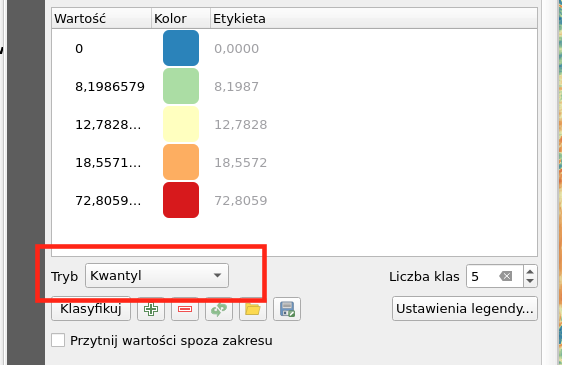
\includegraphics[width=6cm]{nmt-nachylenie-kwantyl}
	\caption{Tryb klasyfikacji - kwantyl}
\end{figure}
		\section{Mapa ekspozycji}
		Drugi ze wskaźników który chciałbym przedstawić to mapa ekspozycji. Przy pomocy takich samych algorytmów matematycznych oraz opcji wyliczany jest dominujący kierunek pomiędzy badaną komórką rastra a czterema lub osmioma sąsiednimi. Kierunek ten może być wyrażony w stopniach liczonych od 0\degree w kierunku północnym, zgodnie ze wskazówkami zegara. Istnieje również możliwość wyliczenia wartości wyrażonej jako sinus kąta.
		\begin{figure}[!ht]
			\centering
			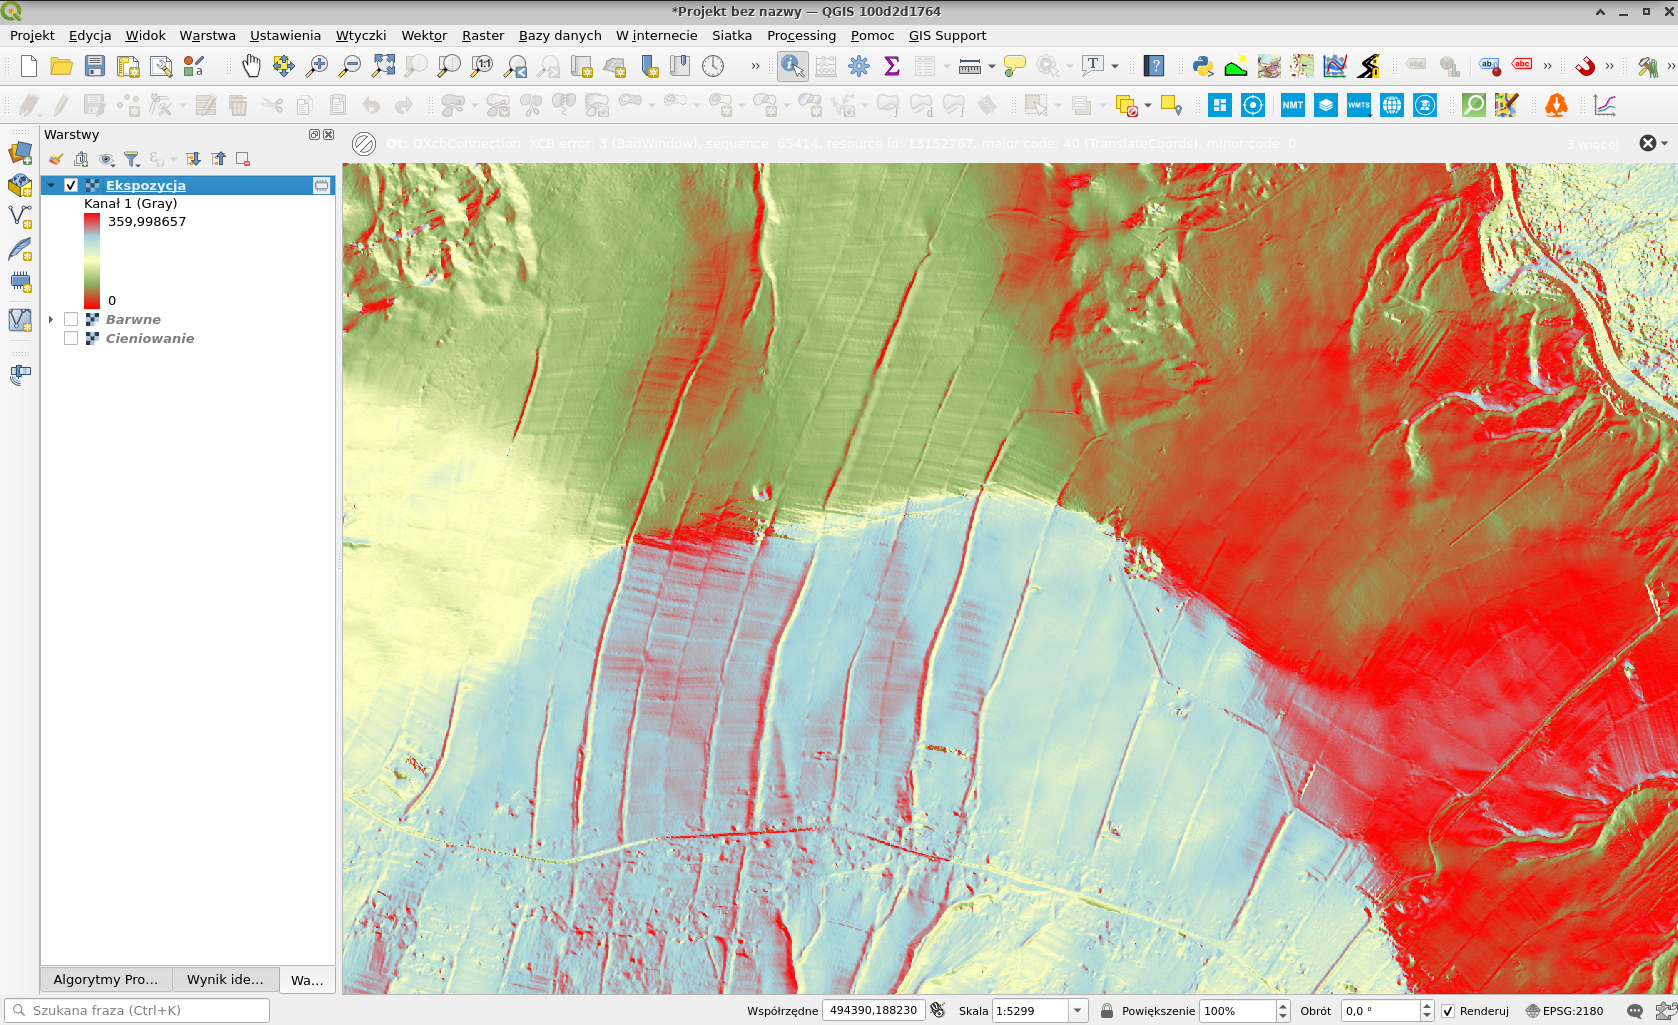
\includegraphics[width=10cm]{nmt-ekspozycja}
			\caption{Mapa ekspozycji}
		\end{figure}
		\section{Inne wskaźniki topograficzne}
		Wśród setek algorytmów i wskaźników topograficznych spróbujmy wskazać te które w najprostszy sposób opiszą nam przestrzeń.
		\section{Ćwiczenia}
			\subsection{Wyznaczenie strefy narażonej osuwiskowo}
			\subsection{Stok narciarski}
	Wyszukanie stoku o ekspozycji północnej oraz nachylonego 10-30 stopni, wykorzystanie fuzzy logic. W tym celu wykorzystamy model numeryczny dla gminy Istebna.
	\begin{enumerate}
	\item W czystym projekcie dodajemy warstwę wirtualnego rastra z katalogu /modul2/nmt/stok
	\item Wykonujemy analizę mapy spadków (nachylenia), przy pomocy narzędzi Geoprocessingu. W zakładce Processing wyszukujemy grupę GDAL, następnie Raster - Analiza. Ustawienia domyślne są wystarczające dla naszych potrzeb.
	\item Następnie przygotowujemy mapę ekspozycji stoku - w grupie GDAL odszukujemy narzędzia Ekspozycja i również stosujemy ustawienia domyślne.
	\item Tak przygotowane mapy posłużą nam jako wejście do algorytmu Fuzzify Raster (Gausian Membership). Function Midpoint ustawiamy w przypadku nachylenia na 23 stopnie, zaś function spread możemy regulować w zakresie 0-1. Spróbujmy ustawić wartość 0,07 (siedem setnych). Im wartość niższa, tym łagodniejszy dzwon Gaussa.
	\item Rastry wyjściowe po funkcji Fuzzy możemy teraz dodać do siebie Kalkulatorem rastra
	\item W ostatnim kroku przy pomocy narzędzi r.to.vect zamienimy mapę rastrową na wektorową.
\end{enumerate}
	\chapter{Widocznosc obiektów}
\section{Dominanty krajobrazu}
\section{Osie widokowe}
\section{Ćwiczenia}

\chapter{Nasłonecznienie}
\section{Mapa nasłonecznienia}
\section{Zmiana warunków}
\section{Potencjał solarny}
\section{Ćwiczenia}
\subsection{Strefy cienia}
\subsection{Jakość powierzchni dachowych dla fotowoltaiki}

\chapter{Wskaźniki urbanizacyjne}
\section{Powierzchnia zabudowy}
\section{Wskaźnik intensywności zabudowy}
\section{Powierzchnia biologicznie czynna}
\section{Ćwiczenia}
\subsection{Wyliczanie powierzchni zabudowy}

\chapter{Publikacja w internecie}
\section{GeoPDF}
\section{Strona html z osadzoną mapą}
\section{Geoportal Lizmap/QWC}
\section{Usługi w chmurze}
\section{Ćwiczenia}
\subsection{Nowa droga rowerowa}
\subsection{Plan zagospodarowania}
\backmatter

\tableofcontents*
\clearpage
%%% BIBLIOGRAPHY
%%% -------------------------------------------------------------

\bibliographystyle{abbrvnat}
\bibliography{qgis}

\end{document}
